\documentclass[10pt,twocolumn,letterpaper]{article}

\usepackage[margin=0.75in]{geometry}
\usepackage{times}
\usepackage{graphicx}
\usepackage{amsmath,amssymb}
\usepackage{booktabs}
\usepackage{multirow}
\usepackage{url}
\usepackage[normalem]{ulem}
\usepackage{xcolor}
\usepackage{tikz}
\usetikzlibrary{shapes.geometric,arrows.meta,positioning,fit,backgrounds,calc}
\usepackage[hidelinks,breaklinks=true]{hyperref}
\usepackage{caption}
\captionsetup{font=small,labelfont=bf}

\setlength{\parskip}{0pt}
\setlength{\columnsep}{0.28in}

\title{\vspace{-1.2em}\textbf{BIM-Graphs: A Literature Review of Hybrid\\
Building-Information Scene Graphs for Robot\\
Navigation and Spatial Question Answering}\vspace{-0.4em}}

\author{Ashwin Nedungadi\\
\small Phase 1 Technical Report --- Literature Review \& Design Reverse-Engineering\\
\small \today
\vspace{-1.5em}}

\date{}

\begin{document}
\maketitle

\begin{abstract}
\noindent
3D scene graphs have become the dominant abstraction for hierarchical spatial
reasoning in robotics, yet nearly all of them are built \emph{bottom-up} from
noisy onboard perception. Building Information Models (BIM), distributed as
Industry Foundation Classes (IFC) files, already encode the metric, semantic and
topological structure that such pipelines spend enormous effort estimating ---
and they do so before a robot has ever entered the building. This review surveys
the two literatures that BIM-Graphs sits between: sensor-driven 3D scene graph
construction, and BIM/IFC semantic modelling. We argue that the naive assumption
underlying most BIM-to-graph work --- that IFC's spatial decomposition tree is
complete and trustworthy --- is empirically false. An audit of 25 real building
models (257\,MB of IFC) finds \textbf{zero} \texttt{IfcRelSpaceBoundary}
instances, only half of storeys containing any \texttt{IfcSpace}, and only 12\%
of elements assigned to a room. We conclude that the central research problem is
not \emph{translation} of IFC into a graph, but \emph{recovery} of the topology
that IFC omits. We then implement the recovery pipeline this implies and report
what breaks: it produces 1{,}025 rooms (344 reconstructed) across the corpus and
satisfies four necessary conditions universally, while exposing five pathologies
of real IFC exports that the surveyed literature does not discuss. Because
necessary conditions can falsify a graph but never confirm it, we identify
ground-truth annotation as the binding constraint on further progress, and
specify a correction-based protocol for obtaining it. An appendix
reverse-engineers the design of the most relevant pipelines and identifies which
of their components transfer to the BIM setting and under what conditions.
\end{abstract}

\section{Introduction}

A 3D scene graph represents an environment as a layered graph whose nodes are
spatial concepts at increasing levels of abstraction --- geometry, objects,
places, rooms, buildings --- and whose edges encode relations among them
\cite{armeni20193d,rosinol2021kimera}. The representation has proven unusually
durable: it compresses dense geometry into something a planner can search
\cite{ray2024tamp}, and something a language model can read without exhausting
its context window \cite{rana2023sayplan}.

The overwhelming majority of this work assumes the graph must be \emph{built by
the robot}. Kimera \cite{rosinol2021kimera} and Hydra \cite{hughes2022hydra}
derive rooms and places from an incrementally reconstructed mesh; S-Graphs
\cite{bavle2022sgraphs,bavle2022sgraphsplus} co-optimises the graph with the
robot's pose; ConceptGraphs \cite{gu2023conceptgraphs} and HOV-SG
\cite{werby2024hovsg} attach open-vocabulary features to segments recovered from
RGB-D streams. This is the right design when no prior exists. For the built
environment, however, a prior almost always does exist. Commercial buildings are
designed in BIM authoring tools and delivered as IFC \cite{buildingsmart_ifc4},
a schema that already contains storeys, rooms, doors, walls, materials and
exact world-frame geometry.

The apparent conclusion --- that BIM makes scene graph construction trivial ---
is the misconception this review is written to dismantle. Exported IFC is a
\emph{drawing-production} artefact, not a topological one. The relationships a
robot needs (which rooms are adjacent, which door connects which pair of rooms,
which room contains which object) are precisely the relationships that authoring
tools omit, because no drawing requires them. Section~\ref{sec:gap} quantifies
this on real data.

\medskip\noindent\textbf{Scope.} We review four clusters:
sensor-driven scene graphs (\S\ref{sec:sensor}); open-vocabulary and
language-grounded graphs (\S\ref{sec:openvocab}); BIM/IFC as a structured prior
(\S\ref{sec:bim}); and space-boundary and room-recovery methods
(\S\ref{sec:rooms}). \S\ref{sec:gap} synthesises these into the gap BIM-Graphs
targets. Appendix~\ref{sec:appendix} reverse-engineers the individual pipeline
components.

\section{Sensor-Driven 3D Scene Graphs}
\label{sec:sensor}

Armeni et al.\ \cite{armeni20193d} introduced the modern formulation: a
four-layer graph over camera, object, room and building, constructed
semi-automatically from panoramic scans of real buildings. The contribution was
the \emph{structure}, not the estimator, and that structure --- objects nested in
rooms nested in a building --- has been inherited almost unchanged by everything
since.

Kimera \cite{rosinol2021kimera} made construction fully automatic from
visual-inertial data, producing a five-layer Dynamic Scene Graph (mesh, objects
and agents, places, rooms, building). Its decisive design choice was to derive
the \emph{places} layer from a Generalised Voronoi Diagram of free space, then
segment rooms by detecting the narrow constrictions --- doorways --- that
separate Voronoi regions. Hydra \cite{hughes2022hydra} made this real-time and,
critically, \emph{loop-closure aware}: when the underlying pose graph is
corrected, the entire hierarchy must deform consistently rather than be rebuilt.
Mono-Hydra \cite{udugama2023monohydra} showed the same architecture degrades
gracefully to monocular input.

The S-Graphs line \cite{bavle2022sgraphs,bavle2022sgraphsplus,bavle2025sgraphs2}
takes a different position: rather than treating the hierarchy as a
post-processing product of SLAM, it makes rooms and walls \emph{factors in the
optimisation itself}. A four-wall room imposes a geometric constraint that
measurably improves pose estimates. S-Graphs 2.0 \cite{bavle2025sgraphs2}
exploits the hierarchy for computational gain, marginalising redundant keyframes
within a room and reporting roughly an order-of-magnitude speed-up on
multi-floor scenes.

Two works in this line are unusually close to our problem because they consume
architectural priors directly. Shaheer et al.\
\cite{shaheer2022localization,shaheer2023architectural} localise a robot by
matching its situational graph against a graph extracted from architectural
plans, and Ndulue et al.\ \cite{ndulue2026matching} replace the combinatorial
matcher with a learned, end-to-end differentiable one, reporting
orders-of-magnitude speed-ups at competitive matching quality. These establish
BIM-derived graphs as a \emph{registration target}; they do not address how to
build a reliable graph when the BIM's own topology is missing.

\section{Open-Vocabulary and Language-Grounded Graphs}
\label{sec:openvocab}

Closed label sets are the binding constraint on the systems above. 3DSSG
\cite{wald20203dssg} and SceneGraphFusion \cite{wu2021scenegraphfusion}
established learned semantic scene graph prediction over fixed vocabularies;
Open3DSG \cite{koch2024open3dsg} removed the fixed relation set by distilling
2D vision-language features into a 3D graph encoder and querying a grounded LLM
for open-set predicates. ConceptGraphs \cite{gu2023conceptgraphs} takes the
pragmatic route --- class-agnostic segmentation, CLIP embeddings per segment,
LLM-inferred inter-object relations --- and HOV-SG \cite{werby2024hovsg} adds the
hierarchy back, building floor/room/object levels with open-vocabulary features
at each and a cross-floor Voronoi graph for traversal, reporting a 75\% memory
reduction against dense feature maps. Clio \cite{maggio2024clio} argues the
correct granularity is \emph{task-dependent} and prunes the graph against a
task list using an information-bottleneck criterion --- directly relevant to us,
since a BIM contains vastly more detail than any single robot task needs.

Recent work pushes toward function rather than appearance: functional scene
graphs \cite{hu2026functional} and TB-HSU \cite{xu2024tbhsu} model affordances
and interactions, which is what the BIM-Graphs design specification calls
``semantic injection.'' KeySG \cite{werby2025keysg} avoids explicit pairwise
edges entirely, storing keyframe-grounded multi-level features and retrieving
through a RAG interface --- evidence that the edge set need not be materialised
if retrieval is good enough.

On the reasoning side, SayPlan \cite{rana2023sayplan} demonstrated the property
that motivates our downstream task: an LLM can plan over a building-scale graph
if permitted to \emph{collapse and expand} it, exploring a small subgraph at a
time instead of ingesting the whole scene. 3DGraphLLM
\cite{zemskova20243dgraphllm}, SG-Nav \cite{yin2024sgnav} and MSGNav
\cite{huang2025msgnav} extend graph-conditioned reasoning to grounding and
zero-shot navigation, and multi-robot hierarchical planning
\cite{strader2025multirobot} scales it across agents.

\section{BIM and IFC as a Structured Prior}
\label{sec:bim}

The AEC community arrived at graph representations independently and earlier.
ifcOWL \cite{pauwels2016ifcowl} mechanically maps the IFC EXPRESS schema to OWL,
preserving everything at the cost of a verbose, deeply reified graph that is
awkward to query. The Building Topology Ontology (BOT)
\cite{rasmussen2021bot} responds with a deliberately minimal core --- zones,
storeys, spaces, elements and adjacency --- and is far closer to what a robot
actually needs. The lesson transfers directly: \emph{completeness and
queryability are in tension, and robotics wants the queryable end.}

Recent work couples these graphs to language models. Iranmanesh et al.\
\cite{iranmanesh2025graphrag} convert IFC to a knowledge graph and use an LLM to
emit Cypher, retrieving grounded facts rather than trusting parametric memory ---
the Graph-RAG pattern our specification adopts. Text2BIM \cite{du2024text2bim}
inverts the direction, generating models from text via a multi-agent framework.

Most directly, BIM-Edit \cite{nithyanantham2026bimedit} benchmarks LLMs on
natural-language editing of IFC across 324 tasks, scoring geometric accuracy,
semantic validity and \emph{topological consistency}. Its headline result is
sobering and strongly motivates the present work: the best model reaches only
49.5\% average score, and none fully solves more than 3.4\% of tasks, with
topological instructions the weakest category. Raw IFC is evidently a poor
interface for language models; an explicit, verified topological graph is the
natural remedy.

For navigation specifically, Zhu et al.\ \cite{zhu2025ifcgraph} build a
semantics-based connectivity graph via IFC-Graph, connecting neighbouring spaces
through doors for indoor pathfinding. Gopee et al.\ \cite{gopee2023ifcnav} export
navigation maps, simulation environments and waypoints from IFC to remove the
manual pre-mapping step, and Karimi et al.\ \cite{karimi2021ontology} formalise
the exchange ontologically. Vega Torres et al.\ \cite{vegatorres2023bimlidar}
close the loop by localising a 2D LiDAR against a BIM-derived map for lifelong
navigation. Pix2G \cite{longo2025pix2g} runs the opposite direction in real time
on a NASA JPL NeBula-Spot, producing BIM-like top-down maps and a multi-layer
graph on CPU alone.

Crucially, \textbf{every one of these BIM-to-graph works presumes a
well-formed spatial hierarchy}, typically that \texttt{IfcSpace} entities exist,
are correctly nested under storeys, and are related to bounding elements. Our
audit shows this presumption fails on realistic exports.

\section{Recovering Spaces and Boundaries}
\label{sec:rooms}

The AEC literature has, in fact, long known that IFC space data is unreliable ---
it surfaced first in building-energy simulation, which needs second-level space
boundaries for thermal analysis. Lilis et al.\ \cite{lilis2017spaceboundary}
generate that topology from raw IFC geometry, explicitly handling clash errors,
malformed space volumes and surface-orientation errors. Fichter et al.\
\cite{fichter2021spaceboundary} note plainly that second-level boundaries in IFC
are ``often missing or incorrect'' and that many delivered files lack
\texttt{IfcSpace} entirely, generating the geometry themselves. This literature
is largely unknown in robotics, yet it solves precisely the problem that blocks
BIM-driven scene graphs.

Where spaces are absent altogether, room recovery becomes a segmentation problem.
Bormann et al.\ \cite{bormann2016roomseg} survey and benchmark the four families
--- morphological, distance-transform, Voronoi and feature-based --- on occupancy
grids, and Voronoi methods remain the default (and are what Kimera and Hydra
adopt internally). Ochmann et al.\ \cite{ochmann2016parametric} reconstruct
\emph{volumetric, parametric} building models from point clouds, casting room
labelling as graph-cut energy minimisation over a line arrangement of wall
centre-lines. Their motivation is the same ``double-sided wall'' pathology named
in our design specification: a wall is a solid with two faces, and treating it as
a zero-thickness surface corrupts adjacency. Kim and Min
\cite{kim2024semanticlayering} add an LLM layer on top of geometric segmentation
to assign functional room labels.

\section{Synthesis and Positioning}
\label{sec:gap}

\begin{table}[t]
\centering
\small
\setlength{\tabcolsep}{3.2pt}
\begin{tabular}{lr}
\toprule
\textbf{Property of the 25-model corpus} & \textbf{Value} \\
\midrule
Total IFC volume        & 257\,MB \\
Storeys / rooms / doors & 146 / 681 / 951 \\
\addlinespace
\texttt{IfcRelSpaceBoundary} (any level) & \textbf{0} \\
Storeys containing $\geq 1$ \texttt{IfcSpace} & 74 / 146 (51\%) \\
Models with $<$50\% storey coverage & 10 / 25 \\
Models with \emph{no} \texttt{IfcSpace} at all & 2 / 25 \\
Models with no storey containment at all & 1 / 25 \\
\addlinespace
Elements assigned to a room & 2{,}001 \\
Elements assigned only to a storey & 15{,}349 (88\%) \\
\addlinespace
Rooms carrying a functional label & 671 / 681 (98.5\%) \\
\bottomrule
\end{tabular}
\caption{Schema-level audit of the 25-model test corpus. Not one file in
257\,MB of IFC provides a single space boundary, and half of all storeys contain
no room whatsoever --- yet almost every room that \emph{is} present is
semantically labelled. IFC is a strong source of semantics and a weak source of
topology.}
\label{tab:audit}
\end{table}

Table~\ref{tab:audit} reports our audit. Three findings organise the project.

\medskip\noindent\textbf{(1) Space boundaries do not exist.} Across 257\,MB of
IFC there are zero \texttt{IfcRelSpaceBoundary} instances of any level. The
schema-sanctioned route from a room to its bounding walls, and from a door to
the pair of rooms it joins, is simply unavailable. Every wall--room and
door--room edge must be recovered geometrically. This validates transplanting
the energy-minimisation and boundary-generation machinery of
\cite{lilis2017spaceboundary,ochmann2016parametric} into a robotics pipeline.

\medskip\noindent\textbf{(2) Room coverage is partial and unreliable.} Only 74 of
146 storeys (51\%) contain any \texttt{IfcSpace}; upper storeys and service
levels are routinely unmodelled, 10 of 25 models fall below half coverage, and
two contain no room at all. A pipeline that traverses
\texttt{IfcBuildingStorey}\,$\rightarrow$\,\texttt{IfcSpace} --- as our own design
specification currently proposes --- silently produces an empty graph for the
majority of the building. Geometric room inference is therefore not an optional
fallback but a required stage. Encouragingly, where spaces \emph{are} present
they are well labelled (671/681 carry a functional \texttt{LongName} such as
\textsc{kitchen} or \textsc{staircase}), so the schema is a strong source of
\emph{semantics} even when it is a weak source of \emph{topology} --- a division
of labour that shapes our architecture.

\medskip\noindent\textbf{(3) Containment is nearly absent.} Only 2{,}001 elements
are assigned to a room against 15{,}349 to a storey alone, and one model states
neither. Object-in-room edges --- the backbone of both navigation and spatial QA
--- must be computed, not read. A further hazard compounds this: units are not
reliable either. One model declares no \texttt{IfcUnitAssignment} whatsoever
while its coordinates are in centimetres, so a parser that trusts the declared
unit silently produces rooms $10^4$ times too large.

\medskip\noindent\textbf{Positioning.} BIM-Graphs therefore differs from
sensor-driven pipelines \cite{hughes2022hydra,werby2024hovsg} in that it never
estimates geometry, and from existing BIM-to-graph work
\cite{zhu2025ifcgraph,gopee2023ifcnav} in that it does not assume the topology it
needs is present. It is best understood as a \emph{topology-recovery} system: it
inherits room segmentation from the robotics literature
\cite{bormann2016roomseg}, boundary generation from building simulation
\cite{lilis2017spaceboundary}, hierarchy from Kimera and Hydra
\cite{rosinol2021kimera,hughes2022hydra}, the collapse/expand query interface
from SayPlan \cite{rana2023sayplan}, and the Graph-RAG retrieval pattern from
\cite{iranmanesh2025graphrag}. The value proposition --- a graph that is metrically
exact by construction, with no SLAM drift and no hallucinated objects, yet with
topology guaranteed complete rather than inherited --- is, to our knowledge,
unoccupied. Its natural evaluation targets are robot navigation and the spatial
reasoning tasks on which raw-IFC LLMs demonstrably fail
\cite{nithyanantham2026bimedit}.

\section{Empirical Study: Building the Recovery Pipeline}
\label{sec:empirical}

To test whether the gap identified above is real and tractable, we implemented
the recovery pipeline of Figure~\ref{fig:pipeline} and ran it over the full
25-model corpus. This section reports what actually broke. We include it because
the failure modes are not incidental engineering detail: several are properties
of real IFC exports that any future BIM-to-graph system will meet, and none are
discussed in the literature surveyed above.

\subsection{Results}

All 25 models process end-to-end (median ${\sim}50$\,s per model, CPU only),
yielding \textbf{1{,}025 rooms --- 681 read from IFC and 344 reconstructed
geometrically} --- with 678 resolved door connections and 10{,}796 catalogued
elements. Because no ground-truth scene graph exists for these buildings, which
is the premise of this work, we validate against \emph{necessary conditions}
that any correct building graph must satisfy rather than against a reference.
Four hold universally; connectivity does not (Table~\ref{tab:validation}).

\begin{table}[t]
\centering
\small
\begin{tabular}{llr}
\toprule
& \textbf{Necessary condition} & \textbf{Pass} \\
\midrule
R2 & every door joins exactly two rooms      & \textbf{25/25} \\
R3 & every room has one storey parent        & \textbf{25/25} \\
R4 & areas and storey heights are physical   & \textbf{25/25} \\
R6 & elements lie inside their assigned room & \textbf{25/25} \\
\addlinespace
R1a & intra-storey connectivity $\geq0.90$   & 10/25 \\
R1b & storeys mutually reachable             & 10/24 \\
R5 & element--room coverage $\geq0.50$       & 18/25 \\
\bottomrule
\end{tabular}
\caption{Validation over the 25-model corpus; mean intra-storey connectivity is
0.789. R1b is not applicable to one model, which contains no vertical
circulation of any kind. These are necessary conditions, \emph{not} accuracy:
they can falsify a graph but cannot confirm that a recovered corridor
corresponds to a real one.}
\label{tab:validation}
\end{table}

\subsection{Pathologies of real IFC exports}

Five defects had to be solved before any topology could be recovered. Each is
invisible in the schema and fatal if unhandled.

\medskip\noindent\textbf{(P1) Units are not trustworthy.} One model declares no
\texttt{IfcUnitAssignment} on its \texttt{IfcProject} at all while its
coordinates are in centimetres; geometry kernels then default to metres and
every room emerges $10^4$ times too large. Because a declared unit may be absent
or wrong, we recover it empirically --- floor-to-floor height is physically
bounded to roughly 2--6\,m, which identifies the true unit to within a decimal
power. A related trap: IfcOpenShell already converts geometry to metres, so
applying the file's unit scale a second time silently shrinks millimetre models
by $10^3$.

\medskip\noindent\textbf{(P2) Sibling storeys share GUID prefixes.} Revit
assigns adjacent storeys near-identical \texttt{GlobalId}s (e.g.\
\texttt{1qw8GM0X\ldots es}, \texttt{\ldots ez}, \texttt{\ldots ec}), so keying
derived nodes on a truncated GUID silently \emph{merges rooms across floors}.
This failure is especially treacherous because it \emph{raises} apparent
connectivity while destroying the hierarchy --- a metric improving for a bad
reason.

\medskip\noindent\textbf{(P3) Doors are barriers first, connections second.}
IFC models doors as solids filling their openings. Rasterising them \emph{closed}
is what makes the connected components of free space separate cleanly into
rooms; door connectivity is restored afterwards by probing along each door's
placement normal. Under world-coordinate tessellation the shape transform is
reported as identity, so that normal must be read from the placement, not the
shape.

\medskip\noindent\textbf{(P4) Not every transition is a door.} Open stairs,
archways and open-plan thresholds carry no \texttt{IfcDoor}. Relying on doors
alone left the entire ground floor of one model unreachable from the storeys
above. We instead test whether the strip of space between two adjacent rooms is
actually filled by wall solids; a mostly empty gap is a passage. This single
addition moved that model from 0.52 to 1.00 reachability.

\medskip\noindent\textbf{(P5) Rooms are drawn for lettable area, not
circulation.} Where a doorway is open at slice height, the free-space component
spans the corridor \emph{and} the rooms off it. Discarding such a component
because it overlaps stated rooms deletes precisely the corridor that makes those
rooms mutually reachable; subtracting the stated rooms instead leaves the
corridor behind. On one model this raised resolved doors from 14 to 32 and
reachability from 0.92 to 1.00.

\subsection{What the residual failures indicate}

The remaining failures are concentrated and informative. Intra-storey
connectivity (R1a) fails predominantly on \emph{open-plan, glazed} buildings
whose enclosure is curtain wall rather than \texttt{IfcWall} --- one model holds
2{,}098 \texttt{IfcPlate} against 51 \texttt{IfcWall} --- where there are few
partitions to recover at all. This is a genuine limitation of occupancy-slice
segmentation inherited from \cite{bormann2016roomseg}, not a tuning artefact.

Several R1b failures are not attributable to the method: one model contains zero
\texttt{IfcStair}, \texttt{IfcRamp} and \texttt{IfcTransportElement} across seven
storeys, each of which is perfectly connected internally but cannot be joined by
any means. We record such cases as not-applicable rather than failed, since
scoring a recovery method on topology the source never contained measures the
wrong thing.

Diagnosis depended on inspecting \emph{what} the isolated rooms were, not the
aggregate. They proved to be bathrooms, hallways, offices and kitchens of median
area 13\,m$^2$; isolated \emph{hallways} are self-evidently wrong, and that is
what pointed to P5. The aggregate alone would merely have suggested a threshold
to tune.

\subsection{Consequence: ground truth is the bottleneck}
\label{sec:bottleneck}

Necessary conditions can falsify a graph but never confirm one. Nothing in
Table~\ref{tab:validation} establishes that a recovered corridor corresponds to
a real one, and precision/recall over rooms and connectivity edges cannot be
computed without annotation. A hand-annotated subset is therefore the critical
next step and the principal obstacle to any quantitative claim; we are building
a correction-based annotation tool (Appendix~\ref{sec:annotation}) for that
purpose.

\bibliographystyle{ieeetr}
\bibliography{bibliography}

\clearpage
\onecolumn
\appendix

\section{Design Breakdown: Reverse-Engineering the Pipelines}
\label{sec:appendix}

This appendix decomposes the most relevant systems into their constituent design
decisions, states the context in which each decision is sound, and records
whether it transfers to the BIM setting.

\subsection{The canonical layered architecture}

Essentially every system in \S\ref{sec:sensor} instantiates the same skeleton.
Figure~\ref{fig:layers} shows it alongside the BIM-Graphs variant.

\begin{figure}[h]
\centering
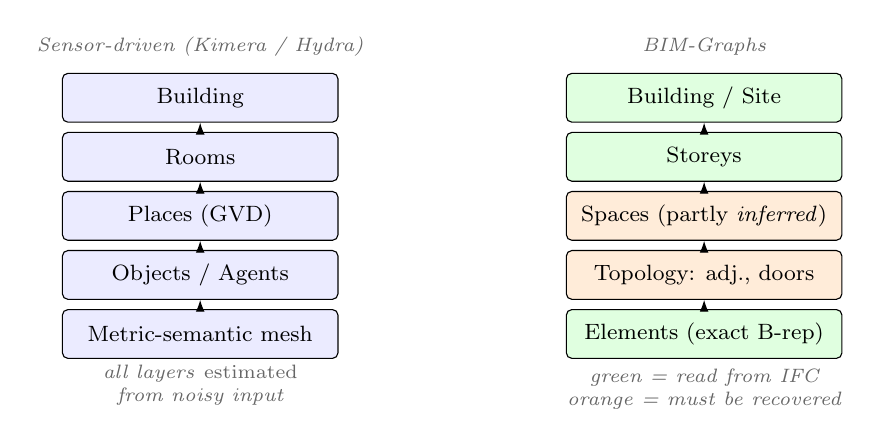
\begin{tikzpicture}[
  font=\footnotesize,
  layer/.style={draw,rounded corners=2pt,minimum width=3.5cm,minimum height=0.62cm,align=center},
  sensed/.style={layer,fill=blue!8},
  given/.style={layer,fill=green!12},
  derived/.style={layer,fill=orange!15},
  lbl/.style={font=\scriptsize\itshape,text=black!60}
]
% Left: sensor-driven
\node[lbl] at (0,0.85) {Sensor-driven (Kimera / Hydra)};
\node[sensed] (a5) at (0,0.2)  {Building};
\node[sensed] (a4) at (0,-0.55) {Rooms};
\node[sensed] (a3) at (0,-1.3) {Places (GVD)};
\node[sensed] (a2) at (0,-2.05) {Objects / Agents};
\node[sensed] (a1) at (0,-2.8) {Metric-semantic mesh};
\draw[-{Latex[length=1.5mm]}] (a1)--(a2); \draw[-{Latex[length=1.5mm]}] (a2)--(a3);
\draw[-{Latex[length=1.5mm]}] (a3)--(a4); \draw[-{Latex[length=1.5mm]}] (a4)--(a5);
\node[lbl,align=center] at (0,-3.45) {all layers \emph{estimated}\\from noisy input};

% Right: BIM-Graphs
\node[lbl] at (6.4,0.85) {BIM-Graphs};
\node[given]   (b5) at (6.4,0.2)  {Building / Site};
\node[given]   (b4) at (6.4,-0.55) {Storeys};
\node[derived] (b3) at (6.4,-1.3) {Spaces (partly \emph{inferred})};
\node[derived] (b2) at (6.4,-2.05) {Topology: adj., doors};
\node[given]   (b1) at (6.4,-2.8) {Elements (exact B-rep)};
\draw[-{Latex[length=1.5mm]}] (b1)--(b2); \draw[-{Latex[length=1.5mm]}] (b2)--(b3);
\draw[-{Latex[length=1.5mm]}] (b3)--(b4); \draw[-{Latex[length=1.5mm]}] (b4)--(b5);
\node[lbl,align=center] at (6.4,-3.5) {green = read from IFC\\orange = must be recovered};
\end{tikzpicture}
\caption{The shared layered skeleton. In sensor-driven systems every layer is
estimated; in BIM-Graphs the outer layers are exact and the \emph{middle} of the
hierarchy --- exactly the part robots need --- is what goes missing.}
\label{fig:layers}
\end{figure}

\noindent\textbf{Why the inversion matters.} Sensor pipelines are most confident
at the top (a building is a building) and least confident at the bottom (is that
a chair?). IFC inverts this: element geometry and class are authoritative, while
the room layer is unreliable or absent. Design effort must therefore be spent in
the opposite place from where the robotics literature spends it.

\subsection{Component-level breakdown}

\begingroup
\centering
\small
\begin{tabular}{p{2.45cm} p{3.5cm} p{4.6cm} p{4.6cm}}
\toprule
\textbf{Component} & \textbf{Origin} & \textbf{Why it works there} & \textbf{Transfer to BIM-Graphs} \\
\midrule
GVD / Voronoi place graph &
Kimera \cite{rosinol2021kimera}, Hydra \cite{hughes2022hydra}, HOV-SG \cite{werby2024hovsg} &
Free space is the only reliable signal from an occupancy map; doorway
constrictions appear as Voronoi bottlenecks, giving room cuts for free. &
\textbf{Transfers, with a better input.} We can rasterise exact free space from
IFC solids instead of a noisy map, so the ``pinch point'' heuristic becomes
near-exact. Primary tool for storeys lacking \texttt{IfcSpace}. \\
\addlinespace
Rooms as optimisation factors &
S-Graphs \cite{bavle2022sgraphsplus,bavle2025sgraphs2} &
A room constrains four wall planes, so asserting it reduces pose drift; the
hierarchy also permits marginalising redundant keyframes. &
\textbf{Does not transfer as stated} --- there is no pose to optimise. The
\emph{hierarchical marginalisation} idea does transfer as a query-time
optimisation for large graphs. \\
\addlinespace
Loop-closure-aware hierarchy &
Hydra \cite{hughes2022hydra} &
Deforming the whole graph on loop closure avoids costly rebuilds. &
\textbf{Not applicable.} No drift, no loop closure. This is precisely the
complexity BIM lets us delete. \\
\addlinespace
Volumetric walls + graph-cut room labelling &
Ochmann \cite{ochmann2016parametric} &
Enforces that walls are solids shared between two rooms, keeping topology
consistent and resolving double-sided surfaces. &
\textbf{Transfers directly}, and answers the ``double-sided wall'' issue named in
our specification. IFC already gives thickness, so the hard estimation step is
skipped. \\
\addlinespace
2nd-level space boundary generation &
Lilis \cite{lilis2017spaceboundary}, Fichter \cite{fichter2021spaceboundary} &
Energy simulation needs surface-exact room boundaries; the methods are built
assuming IFC data is broken. &
\textbf{Core import.} This is the closest existing solution to our
\texttt{IfcRelSpaceBoundary}${=}0$ problem and is under-cited in robotics. \\
\addlinespace
Door-mediated space connectivity &
IFC-Graph \cite{zhu2025ifcgraph}, IndoorGML-style models &
Doors are the only legitimate inter-room transitions, so the navigation graph is
spaces-as-nodes, doors-as-edges. &
\textbf{Transfers, but must be earned.} Without space boundaries we must resolve
each door's two adjoining rooms geometrically, by casting along the door normal. \\
\addlinespace
Open-vocab.\ features per node &
ConceptGraphs \cite{gu2023conceptgraphs}, Open3DSG \cite{koch2024open3dsg} &
Recovers semantics a closed detector misses; CLIP embeddings make nodes
queryable by text. &
\textbf{Partly redundant.} IFC already names elements and labels 149/155 rooms.
Worth reserving for \emph{affordances}, which IFC never encodes. \\
\addlinespace
Task-driven pruning &
Clio \cite{maggio2024clio} &
Task-agnostic graphs are needlessly large; an information-bottleneck criterion
keeps only task-relevant granularity. &
\textbf{Highly relevant.} A single IFC yields $10^4$--$10^5$ entities, most of
them irrelevant (individual curtain-wall mullions). Pruning is a necessity. \\
\addlinespace
Collapse/expand LLM interface &
SayPlan \cite{rana2023sayplan} &
Keeps building-scale graphs inside a context window by exposing one subgraph at
a time. &
\textbf{Transfers directly} and is the intended shape of our QnA interface. \\
\addlinespace
Text-to-Cypher Graph-RAG &
\cite{iranmanesh2025graphrag} &
Grounds answers in retrieved triples rather than parametric memory, reducing
hallucination. &
\textbf{Adopted} by the design specification; complements rather than replaces
collapse/expand. \\
\bottomrule
\end{tabular}
\captionof{table}{Reverse-engineered components, the context that justifies each,
and whether it survives the move from sensor data to BIM.}
\label{tab:components}
\par\endgroup
\medskip

\subsection{The recovery pipeline implied by the analysis}

Combining the transferable components yields the design in
Figure~\ref{fig:pipeline}: read what IFC states, then recover what it omits, and
only then attach open-vocabulary semantics.

\begin{figure}[h]
\centering
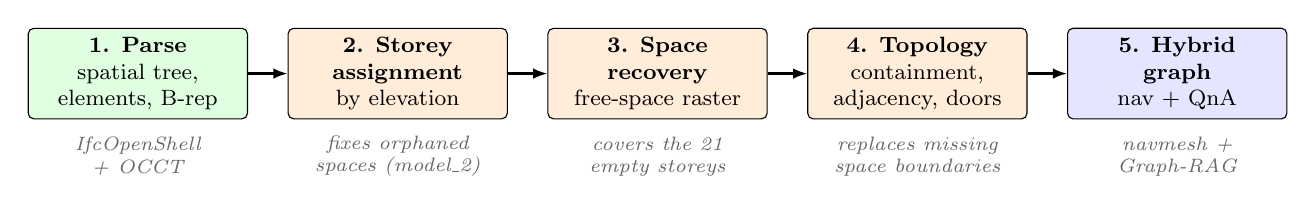
\begin{tikzpicture}[
  font=\footnotesize,
  box/.style={draw,rounded corners=2pt,minimum height=0.95cm,text width=2.55cm,align=center},
  readbox/.style={box,fill=green!12},
  recbox/.style={box,fill=orange!15},
  outbox/.style={box,fill=blue!10},
  ar/.style={-{Latex[length=1.8mm]},thick}
]
\node[readbox] (p1) at (0,0)    {\textbf{1. Parse}\\spatial tree,\\elements, B-rep};
\node[recbox]  (p2) at (3.3,0)  {\textbf{2. Storey\\assignment}\\by elevation};
\node[recbox]  (p3) at (6.6,0)  {\textbf{3. Space\\recovery}\\free-space raster};
\node[recbox]  (p4) at (9.9,0)  {\textbf{4. Topology}\\containment,\\adjacency, doors};
\node[outbox]  (p5) at (13.2,0) {\textbf{5. Hybrid\\graph}\\nav + QnA};
\draw[ar] (p1)--(p2); \draw[ar] (p2)--(p3); \draw[ar] (p3)--(p4); \draw[ar] (p4)--(p5);
\node[font=\scriptsize\itshape,text=black!60,align=center] at (0,-1.05) {IfcOpenShell\\+ OCCT};
\node[font=\scriptsize\itshape,text=black!60,align=center] at (3.3,-1.05) {fixes orphaned\\spaces (model\_2)};
\node[font=\scriptsize\itshape,text=black!60,align=center] at (6.6,-1.05) {covers the 21\\empty storeys};
\node[font=\scriptsize\itshape,text=black!60,align=center] at (9.9,-1.05) {replaces missing\\space boundaries};
\node[font=\scriptsize\itshape,text=black!60,align=center] at (13.2,-1.05) {navmesh +\\Graph-RAG};
\end{tikzpicture}
\caption{The pipeline implied by the gap analysis. Green is read from IFC; orange
is recovered; blue is the deliverable. Stages 2--4 are the research contribution
and are exactly the stages the original design specification assumed away.}
\label{fig:pipeline}
\end{figure}

\subsection{Consequences for the original design specification}

The reverse-engineering exercise suggests three amendments to
\texttt{Hybrid\_BIM2Graph\_Design\_Spec}:

\begin{enumerate}\itemsep2pt
\item \textbf{The traversal
\texttt{IfcProject}$\rightarrow$\texttt{IfcBuildingStorey}$\rightarrow$\texttt{IfcSpace}$\rightarrow$\texttt{IfcProduct}
is not viable as the primary path.} It yields nothing for 21 of 35 storeys and
nothing at all for model\_2. It should be demoted to a \emph{fast path} with
geometric recovery as the guaranteed fallback.
\item \textbf{Double-sided wall handling should follow Ochmann
\cite{ochmann2016parametric} rather than normal-duplication.} Duplicating
boundaries along the thickness vector re-derives, less robustly, a volumetric
representation IFC already provides explicitly.
\item \textbf{Stage 2/3 rendering is not on the critical path.} Because IFC
labels 671/681 rooms and names every element, a metrically exact and
topologically complete graph is attainable with no rendering whatsoever. VLM
injection should be scoped to affordances --- the one thing IFC genuinely lacks
--- rather than treated as a prerequisite for graph construction. The
implementation in \S\ref{sec:empirical} confirms this: the full graph, including
navigation and QnA interfaces, was produced without rendering a single frame.
\end{enumerate}

\section{Annotation Protocol for Ground Truth}
\label{sec:annotation}

\S\ref{sec:bottleneck} identifies annotation as the binding constraint. Because
annotating 25 buildings from scratch is prohibitive, we annotate \emph{by
correction}: the pipeline's prediction is displayed over the true floor plan and
the annotator adjudicates it. This converts an open-ended drawing task into a
sequence of bounded judgements, and yields exactly the quantities the necessary
conditions cannot supply.

\subsection{What is annotated}

\begin{enumerate}\itemsep2pt
\item \textbf{Room verdicts.} Each predicted room is marked \textsc{correct},
\textsc{spurious} (not a real room --- a shaft, void or artefact),
\textsc{merge} (two predictions that are one room) or \textsc{split} (one
prediction covering several). A corrected functional label may be supplied,
which also gives ground truth for semantic labelling.
\item \textbf{Missing rooms.} A real room the pipeline failed to find is marked
by placing a point inside it and labelling it. A point suffices for recall; a
polygon is optional, since exact boundaries are rarely in dispute.
\item \textbf{Connection verdicts.} Each predicted \texttt{connected\_by\_door},
\texttt{open\_passage} and \texttt{vertically\_connected} edge is confirmed or
rejected, and missing connections are added by selecting two rooms. This is the
critical annotation: connectivity is what the schema omits entirely and what
navigation depends on.
\end{enumerate}

\subsection{Metrics it enables}

Room precision/recall and connectivity precision/recall follow directly, both
reportable separately for rooms \emph{stated} by IFC versus rooms
\emph{recovered} geometrically --- the comparison that isolates the contribution
of the recovery stage from what the file already provided. Label accuracy over
corrected functional names measures the semantic layer. Together these replace
the necessary conditions of Table~\ref{tab:validation} with genuine accuracy.

\subsection{Design constraints}

Three properties matter for a tool that colleagues will actually use. It must
open an IFC and show a floor plan in seconds, so geometry is pre-extracted and
cached rather than tessellated on demand. Every judgement must be one click,
with keyboard shortcuts for the common verdicts. And annotations must be stored
per annotator, so that the same model can be labelled independently by two
people and inter-annotator agreement measured --- without which we cannot know
whether disputed corridors reflect pipeline error or genuine ambiguity about
where one room ends and the next begins.

\end{document}
